\section{Results}
\label{sec:results}

\subsection{Genetic Correlation}
\label{sub:psych_genetic_correlation}

First, the genetic correlations between impulsive aggression and depressive symptoms is remarkably high ($r_g=0.6741$, $SE=0.0919$, $p=2.2326\times 10^{-13}$).
This high correlation is also reflected in subjects diagnosed with a major depression ($r_g=0.4134$, $SE=0.1212$, $p=6\times 10^{-04}$).
In contrast, correlations between impulsive aggression and Bipolar disorder was not significant after adjusting for multiple testing at $\alpha=0.00625$ ($r_g=0.1192$, $SE=0.0949$, $p=0.2091$).
Similar genetic correlations with Schizophrenia was not of large effect ($r_g=0.161$, $SE=0.0566$, $p=0.0045$) and failed to pass multiple testing.

In contrast correlations between risk taking and Bipolar ($r_g=0.2561$, $SE=0.0606$, $p=2.4034\times 10^{-05}$), as well as Schizophrenia ($r_g=0.232$, $SE=0.0431$, $p=7.3554\times 10^{-08}$) remained significant.
In addition, while genetic correlations were highly significant between aggression and depression, genetic correlations between risk raking, depressive symptoms ($r_g=0.0856$, $SE=0.0687$, $p=0.2129$) as well as MDD ($r_g=0.0028$, $SE=0.0853$, $p=0.974$) were small and did not pass the multiple testing threshold.

An overall overview of all genetic correlations are given in Figure~\ref{fig:figures/combined_corr.pdf}.

\begin{figure}[htpb]
  \centering
  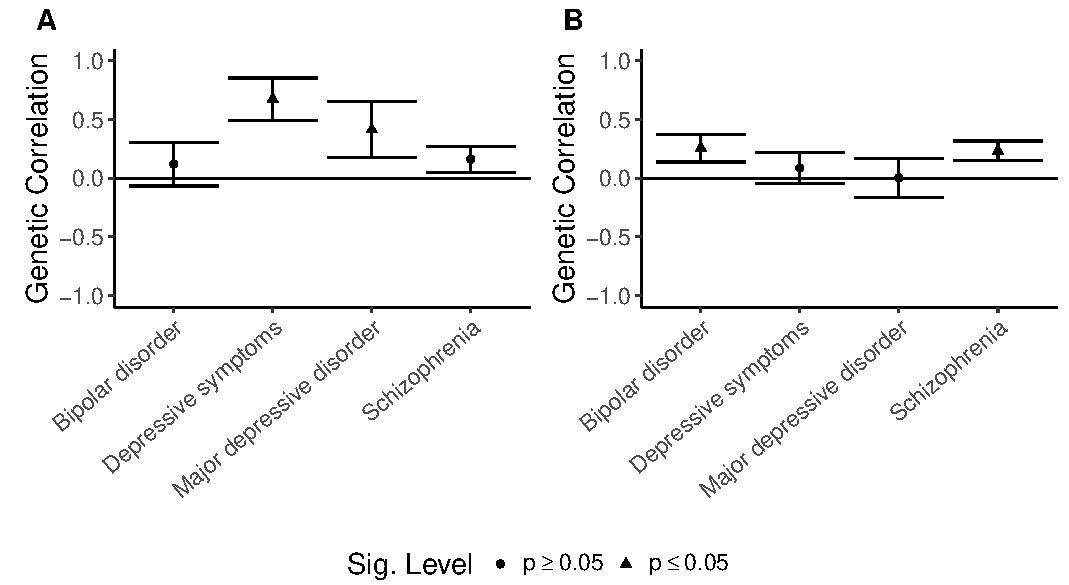
\includegraphics[width=0.8\linewidth]{figures/combined_corr.pdf}
  \caption{Genetic correlations between impulsive aggression and risk taking with selected psychiatric disorders.
    The error bars display the 95\% confidence intervals for each pairwise genetic correlations.
    Significance levels after multiple testing correction are displayed in form of a dot ($p\ge 0.05$) and triangle ($p\leq0.05$).
    (A) Genetic correlations between impulsive aggression and psychiatric disorders. 
    (B) Genetic correlations between risk taking and psychiatric disorders.
  }\label{fig:figures/combined_corr}
\end{figure}


\subsection{Mendelian Randomization}
\label{sub:mendelian_randomization}

Utilization of MR to infer potential causal influence of psychiatric disorders on aggression and risk taking yielded two potential links (Figure~\ref{fig:overall_mr_effect}).
While most methods agree with the direction of effect, MR-Egger commonly resulted in larger confidence intervals and did not resulted in any significant findings.
Nevertheless, MR-egger is known to be less powerful in cases where most used genetic variants are valid instruments.

MR analysis suggest some indication that SZ might causally influence both aggression and risk taking.
In particular, all applied methods, with the exception of MR-Egger, support the notion that SZ might both increase levels of risk taking as well as impulsive aggression.
In addition, there is little evidence for a possible MR assumption violation via pleiotropic effects.
Both funnel plots in Figure~\ref{fig:sensitivity} as well as MR-Egger intercepts (Figure~\ref{fig:sensitivity}) suggest little to no pleiotropy between instrument and outcome.
Further, these results seem not to be driven by outliers (see Figure~\ref{fig:mr_aggression} and Figure~\ref{fig:mr_risk}).
This indicates a potential causal effect of SZ on both risk taking and impulsive aggression.

Mixed results were obtained in the MR analysis investigating a potential causal effect of depression on aggressive behavior.
Depressive symptoms are suggested to cause an increase in impulsive aggression by all but MR-egger.
Specifically, MR-Egger regression indicates, while retaining an non-significant slope, the opposite direction of effect compared to other used methods.  
A possible explanation for this discrepancy can be found in potential pleiotropic effects which might violate MR assumptions (see Figure~\ref{fig:sensitivity}).
Indeed, inspection of the funnel plot in Figure~\ref{fig:sensitivity} shows considerable asymetry, thus suggesting the presents of pleiotropic effects.
In addition, the intercept of MR-egger regression differs significantly from $0$.
Thus, there is no evidence which could suggest a causal influence of depressive symptoms on aggression. 
Similar, but weaker, results were obtained from the MR analysis between MDD and impulsive aggression.
None, of the used methods suggested significant causal effects between the two phenotypes. 
Further, analysis of the funnel plot suggest a possible pleiotropy violation.

In addition, there is some indication of a causal effect of BP on risk taking.
However, these effects are rather weak across the used instruments.
Further, MR analysis was unable to identify causal effects of both DS and MDD on risk taking.
Also an effect of BP on impulsive aggression was not supported within this analysis.

\begin{figure}[htpb]
  \centering
  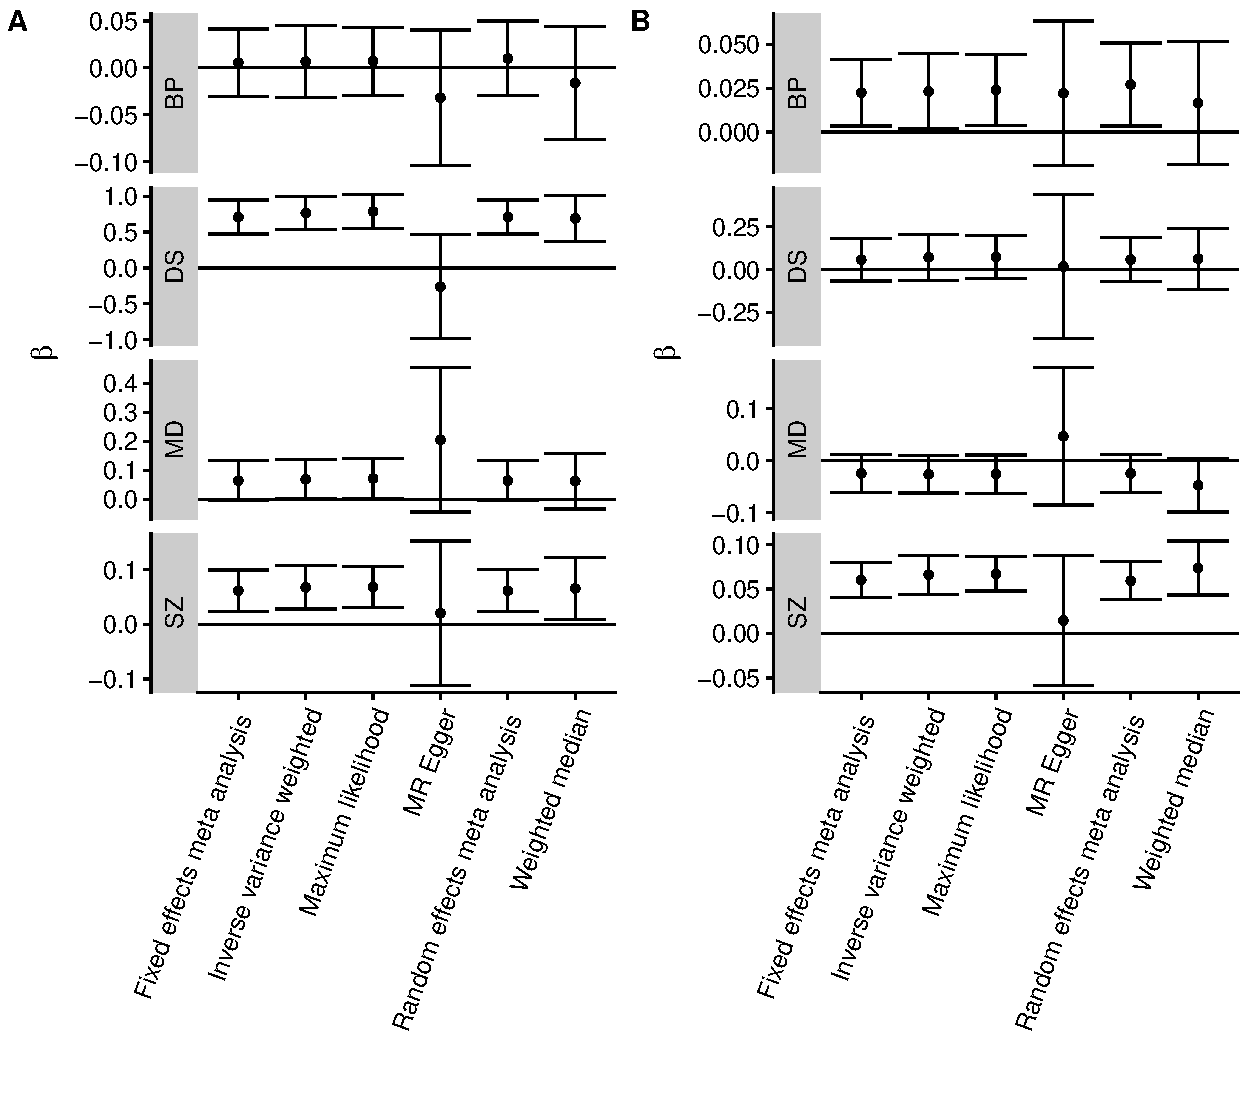
\includegraphics[width=0.9\linewidth]{figures/overall_mr_effect.pdf}
  \caption{Estimated causal effect of psychiatric disorders on impulsive aggression and risk taking.
    The effect size of the causal effect $\beta$ is displayed on the y-axis, while used Mendelian randomization methods are on the x-axis.
    SZ, Schizophrenia; MDD, Major Depressive Disorder; DS, Depressive Symptom's; BP, Bipolar Disorder.
    (A) Effect of psychiatric disorders on impulsive aggression.
    (A) Effect of psychiatric disorders on risk taking.
  }\label{fig:overall_mr_effect}
\end{figure}

\begin{figure}[htpb]
  \centering
  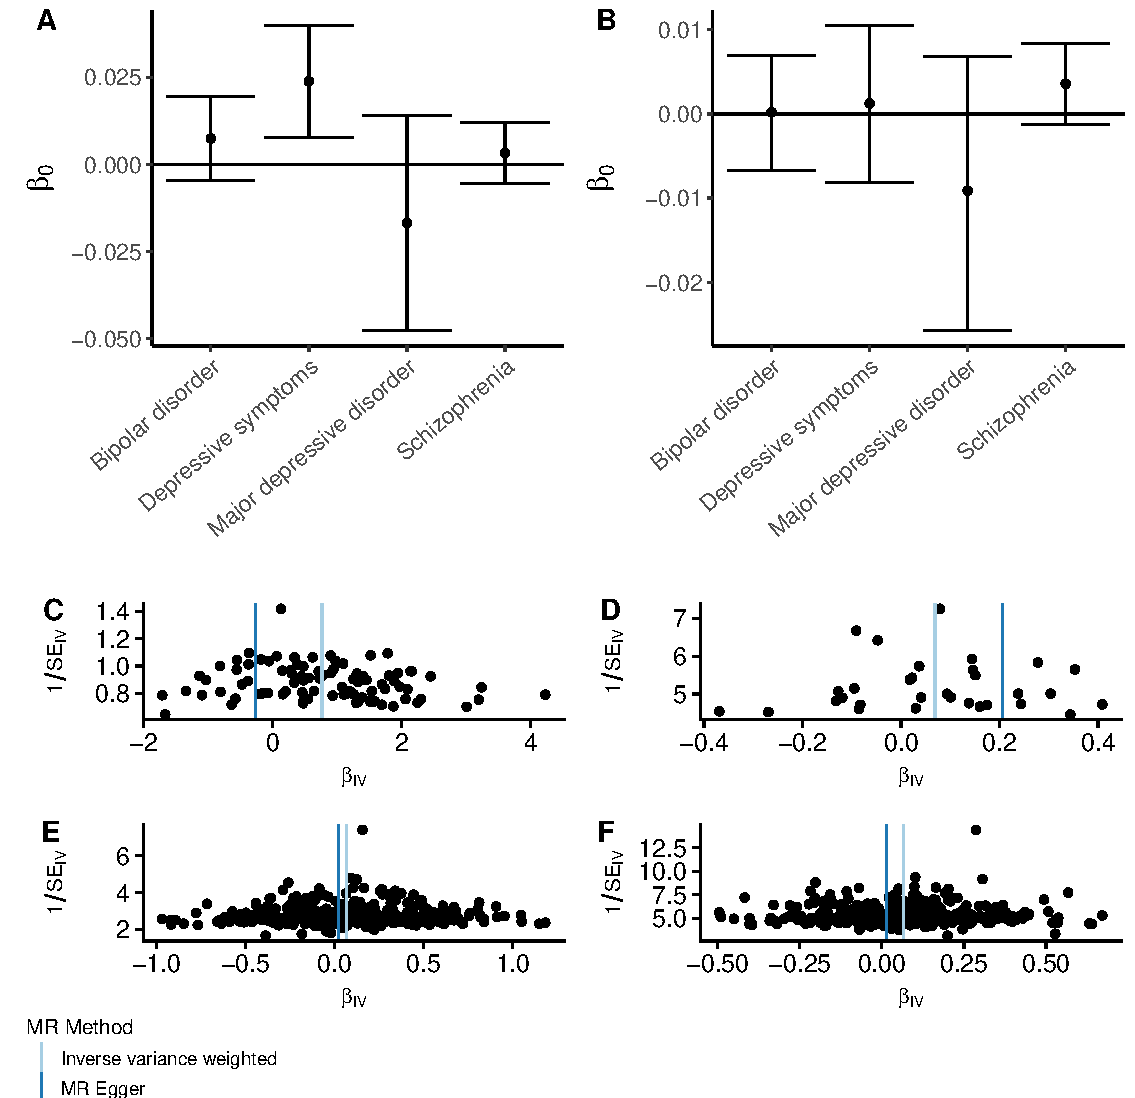
\includegraphics[width=0.9\linewidth]{figures/sensitvity_plot.pdf}
  \caption{Sensitivity analysis.
    (A) Displays the intercept $\beta_0$ of MR-egger regression for psychiatric disorders on impulsive aggression. The intercept is an indication of whether directional horizontal pleiotropy is driving the MR analysis.
    (B) The MR-egger regression intercept of psychiatric disorders on risk taking.
    (C) Funnel plot of Depressive symptoms on impulsive aggression. 
    (D) Funnel plot of MDD on impulsive aggression. 
    (E) Funnel plot of SZ on impulsive aggression. 
    (F) Funnel plot of SZ on risk taking. 
    The intercept of both MR-egger and Inverse variance method are indicated with a vertical line.
    Error bars indicate the 95\% confidence intervals.
  }\label{fig:sensitivity}
\end{figure}

The hypothesised direction between exposure and outcome were tested with the help of the Steiger test~\cite{Steiger1980}.
In general the test examines if the variance explained by the used instrumental SNP in the outcome is less than those within the exposure. 
Careful inspection of these test results suggest that there were no violation of the hypothesised direction of causal effects across all tested connections.

To conclude, careful examination of the here presented MR analysis gives some indication of a causal connection between SZ on both risk taking and impulsive aggression.
However, potential causal effects of other psychiatric disorders on aggression or risk taking was not supported.
